\section{Implementación}\label{implementacionPosta}
Un sistema de captura de movimiento con las características necesarias para cumplir el objetivo de este proyecto debe implementar cuatro bloques generales: \emph{calibración}, \emph{detección de marcadores}, \emph{reconstrucción} y \emph{seguimiento}. En la Figura \ref{bloquesSist} se muestra un esquema del sistema a implementar, cada bloque verde indica la salida de una etapa siendo  a su vez la entrada del bloque siguiente.
%\vspace{-0.6cm}
\begin{figure}[ht!]
	\centering
	\hspace{-0.5cm}
	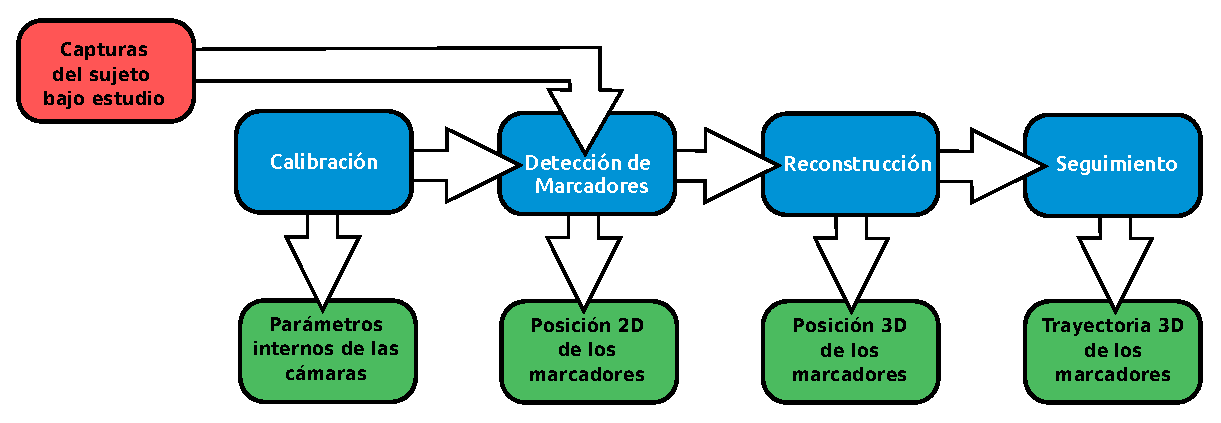
\includegraphics[scale=0.55]{imagenes/Sistema_completo/Diagrama_de_bloques.eps}
	\caption{Diagrama de bloques del sistema completo.}
	\label{bloquesSist}
\end{figure}
%\vspace{-0.7cm}
%Es importante destacar el hecho de poder separar el sistema en bloques independientes,

Es importante destacar la independencia entre bloques, permitiendo modificar u optimizar fácilmente el sistema en etapas futuras.
A continuación se describe el funcionamiento de cada etapa del proceso de captura de movimiento, asi como su implementación.
\subsection{Calibración}\label{calibracion}

%\subsection{Calibración para secuencias reales}

%\label{seccion_calibracion_secuencias_reales}

%%%%%%%%%%%%REFERENCIAS%%%%%%%%%%%%%%%%%
% LIC DARIO SANTOS, HOSPITAL DE CLÍNICAS

%Se ha podido tener acceso a secuencias de video de análisis del movimiento de la marcha que se han realizado en el Hospital de Clínicas. Dichas secuencias han sido obtenidas por un grupo de médicos e investigadores con el objetivo de analizar el movimiento de pacientes en el ámbito terapéutico o con un objetivo esencialmente de investigación desde el punto de vista de la biomecánica.

%DEBERÍA ACLARARSE QUE ESTO SE HACIA ANTES, CREO QUE TIPO POR 2009 Y AHORA USAN VICON.
%\vspace{-0.3cm}
%\begin{figure}[ht!]
%\centering
%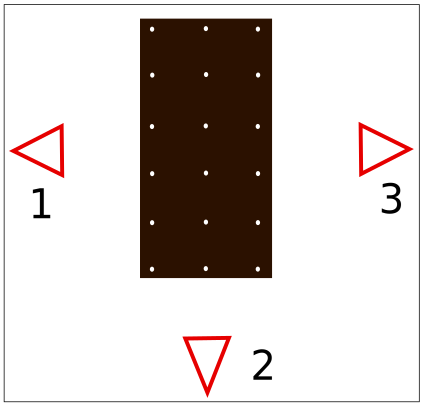
\includegraphics[scale=0.5]{img/calibracion/lab_real.pdf}
%\vspace{-0.3cm}
%\caption{Laboratorio del Hospital de Clínicas.}
%\label{fig: lab_real}
%\end{figure}


%La metodología utilizada consiste en el uso de tres cámaras de video convencionales de 25 fps y resolución  720 x 576 píxeles. Dichas cámaras se disponen como se muestra en la Figura \ref{fig: lab_real}, alrededor de una alfombra o cinta sobre la que se le pide al paciente que camine.\\



%La persona que se desea evaluar debe tener colocados marcadores, fundamentalmente en las articulaciones del cuerpo, y debe desplazarse sobre la alfombra dispuesta para esto. En la Figura \ref{fig: persona con marcadores}, se observa a un individuo caminando con los marcadores colocados.

%\vspace{-0.2cm}
%\begin{figure}[ht!]		
        %\subfloat[Persona con marcadores]{\includegraphics[scale=0.28]{img/calibracion/captura_real.png}\label{fig: persona con marcadores}}
%        \hspace{0.1cm}
        %\subfloat[Objeto de calibración]{\includegraphics[trim = 20mm 0mm 40mm 0mm, clip, scale=0.28]{img/calibracion/calibrador.png}\label{fig: calibrador}}
%  \caption{Captura de secuencia real}
      \label{fig: captura real}
%\end{figure}

%Antes de la captura del movimiento se emite una señal acústica con la cual se sincronizan las tres vistas una vez obtenidos los videos. El software con el cual este grupo de médicos ha analizado el movimiento es el \textit{Dvideow}.            
 %%%%%%%%%%%%%%%%%%(REFERENCIAR)%%%%%%%%%%%%%%%%%%%%%%%%%%%%%%. 
% Dicho software realiza la detección, seguimiento y reconstrucción de los marcadores. Por otro lado, no se ha podido tener acceso a este software por lo cual tampoco se pudo evaluar su desempeño y compararlo con el desarrollado en este proyecto.\\

%El método que utilizaron para calibrar las cámaras requiere de un objeto de calibración como el que se muestra en la Figura \ref{fig: calibrador}, al que se le llama \textit{fantoma}. Este objeto se compone de marcadores colocados sobre una estructura cuyas dimensiones son conocidas. Dicho objeto se lo coloca en posiciones determinadas que se encuentran marcadas sobre la alfombra, ver Figura \ref{fig: calibrador}. De esta manera se obtiene un mayor número de puntos ubicados en el volumen de trabajo.\\


%Los videos proporcionados por los especialistas del Hospital de Clínicas incluyen tanto las secuencias de marcha de diferentes individuos como el proceso con el que se calibran las cámaras del laboratorio. A partir de dichos videos se desarrolló un algoritmo tal que permite extraer las matrices de proyección de cada una de las cámaras. Tomando un cuadro del video en el que se encuentre el \textit{fantoma} en una de las posiciones, el algoritmo implementado requiere que cada marcador del \textit{fantoma}, en cada una de las vistas, sea seleccionado manualmente, y en un orden tal que permita establecerse una correspondencia entre las proyecciones de un mismo marcador en las tres vistas. En la Figura \ref{fig: vistas_calibrador} se muestra a uno de los marcadores seleccionado en cada una de las vistas.
%\vspace{-0.53cm}
%\begin{figure}[ht!]
%        \hspace{-1cm}
        %\subfloat[Vista cámara 1]{\includegraphics[trim = 59mm 0mm 41mm 0mm, clip,scale=0.45]{img/calibracion/calibrador_cam1.png}}
%                \hspace{1mm}
       % \subfloat[Vista cámara 2]{\includegraphics[trim = 50mm 0mm 50mm 0mm, clip,scale=0.45]{img/calibracion/calibrador_cam2.png}}     	
%  \hspace{1mm}
        %\subfloat[Vista cámara 3]{\includegraphics[trim = 32mm 0mm 68mm 0mm, clip,scale=0.45]{img/calibracion/calibrador_cam3.png}}
      
%      \caption{Uno de los marcadores de calibrador seleccionado en cada una de las cámaras}
%      \label{fig: vistas_calibrador}      
%\end{figure}


%Por otra parte la posición de los marcadores en el espacio 3D es conocida ya que se saben las medidas del \textit{fantoma}, ver Figura \ref{fig: medidas_calibrador}. Dichas posiciones pueden ser referidas un punto que puede elegirse arbitrariamente, así como los ejes de coordenadas $(x,y,z)$.

%\vspace{-0.53cm}
%\begin{figure}[ht!]
%        \centering
     %{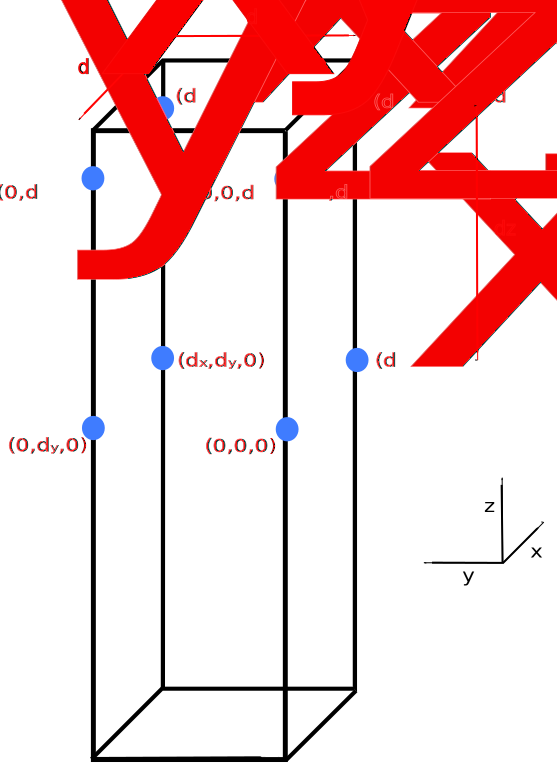
\includegraphics[scale=0.38]{img/calibracion/medidas_calibrador.pdf}}    
%     \caption{Coordenadas de los marcadores del \textit{fantoma}}
%      \label{fig: medidas_calibrador}     
%\end{figure}

%  De esta forma se tiene asociadas las coordenadas 3D de los marcadores en el espacio con sus correspondientes coordenadas 2D en píxeles en cada una de las cámaras, $\mathbf{X_i} \leftrightarrow  \mathbf{x_i}$. Si se tiene una cantidad suficiente de puntos, entonces las matrices de proyección $P$ pueden ser estimadas tal que $\mathbf{x_i}=P\mathbf{X_i}$. Para esto se utiliza el algoritmo \textit{Direct Linear Transformation (DLT)}.\\
   
% Según lo demostrado en \cite{hartley}, para cada asociación de puntos $\mathbf{X_i} \leftrightarrow \mathbf{x_i}$ se cumple que :
   
%   \[
%   \begin{pmatrix}
%   0^T & -w_iX_i^T & y_iX_i^T \\
%   w_iX_i^T & 0^T & -x_iX_i^T
%   \end{pmatrix}
%   \begin{pmatrix}
%    P^1 \\
%    P^2 \\
%    P^3
%   \end{pmatrix}
%   = 0   
%      \]
   
   
% \hspace{-0.6cm}siendo $P^{iT}$ las columnas $i$-ésimas de $P$ y $\mathbf{x_i}$ de coordenadas homogéneas $(x_i,y_i,w_i)$. Dicha matriz se obtiene resolviendo un conjunto de ecuaciones del tipo $Ap=0$.  Dado que por cada punto se tiene dos ecuaciones y que la matriz $P$ tiene doce entradas y once grados de libertad, ignorando el factor de escala, resulta que son necesarios conocer al menos seis correspondencias $X_i \leftrightarrow x_i$.\\
 
%Para anular los efectos de la selección arbitraria del origen y la escala del sistema de coordenadas se aplica una normalización tanto a los puntos imagen 2D como a los 3D, logrando de esta manera mejorar los resultados finales. Para los puntos 2D de cada vista se traslada el origen de coordenadas de dicha vista al centroide de los puntos y se aplica un escalado tal que la distancia promedio de los puntos al origen sea $\sqrt{2}$. Para los puntos 3D el mismo procedimiento excepto que el escalado que se aplica es tal que la distancia promedio al origen es $\sqrt{3}$. De esta manera se tiene dos matrices que realizan esta transformación, la matriz $T_{3D}$ tal que $\tilde{X_i} = T_{3D}^{}X_i$ para los puntos en el espacio, siendo $\tilde{X_i}$ los puntos normalizados. Análogamente para los 2D imagen se tiene la matriz $T_{2D}^{}$ tal que $\tilde{x_i} = T_{2D}^{}x_i$. \\
 
% Dado que las coordenadas de los puntos 2D están afectadas por el ruido y que se tienen más de seis correspondencias $X_i \leftrightarrow x_i$, no existe una solución exacta a las ecuaciones $Ap=0$. Por lo tanto la solución se obtiene minimizando un error, en este caso se busca $p$ tal que minimice $||Ap||$. Para esto se utiliza la descomposición en valores singulares (SVD), donde se obtiene del vector singular asociado al menor valor singular. De esta manera se obtiene la matriz de proyección $\tilde{P}$. Por último debe descomponerse la normalización, por lo tanto la matriz de proyección $P$ queda $P = T_{2D}^{-1} \tilde{P} T_{3D}^{}$.
 
%\subsection{Calibración simulada en \emph{Blender}}
 
 Con el objetivo de establecer una metodología de calibración que fuera válida para la configuración de cámaras con las que se diseñó el entorno virtual descrito en la sección \ref{section_base_de_datos}, se probaron distintas implementaciones existentes. Para esto se evaluaron dos toolbox elaborados en \emph{Matlab}. La metodología de calibración fue simulada en \emph{Blender} mediante \textit{scripts} \emph{Python} y las imágenes obtenidas como resultado se procesaron con dichos toolbox. La descripción de la metodología y las simulaciones se detalla en \cite{proyecto_biomecanica}.\
 
 Uno de los toolbox utilizados es el \textit{Automatic Multi-Camera Calibration Toolbox (amcctoolbox)} \cite{amcctoolbox}, el cual utiliza como objeto de calibración un damero. Este método, aunque sus resultados tienen buena precision \cite{zhang_libro}, puede no ser suficientemente flexible para un sistema de muchas cámaras ya que, entre otras cosas, es necesaria la intervención manual en algunos casos.\
 
El otro toolbox utilizado es el \textit{Multi-Camera Self-Calibration Toolbox} \cite{toolbox_led}. Este método consiste en capturar el movimiento de una fuente puntual de luz que recorra el volumen de trabajo. Para cada cuadro se tiene un punto 3D en el espacio en una posición distinta y en cada una de las cámaras su correspondiente proyección.
 El error de re-proyección promedio obtenido es menor a 0.13 píxeles para todas las cámaras. Este método plantea una forma simple de calibrar un conjunto de muchas cámaras adecuado para el sistema de 17 cámaras del laboratorio virtual desarrollado en \emph{Blender}.

 
 
%\subsubsection{Automatic Multi-Camera Calibration Toolbox (amcctoolbox) }\cite{amcctoolbox}  


%Esta herramienta automatiza ciertas funciones del toolbox \textit{Camera Calibration Toolbox}, reduciendo la intervención del usuario. Utiliza como objeto de calibración un damero.

%Para la calibración de conjuntos de varias cámaras, el damero debe ser colocado en múltiples ubicaciones y orientaciones cubriendo el mayor volumen de trabajo tal que, en cada una de estas posiciones, el damero pueda ser visto por más de una cámara simultáneamente.

%La calibración del entorno virtual se realiza simulando un damero real. Para cada par de cámaras adyacentes se coloca el damero en algún punto dentro del volumen de trabajo, con una orientación tal que la figura plana del damero sea visible en ambas cámaras. Luego, a partir de dicha posición, se toman capturas del damero cambiando ligeramente la ubicación y orientación del mismo. Para cada par de cámaras adyacentes se consideran entre 15 y 20 posiciones distintas del damero.

%Una vez realizadas las capturas se procesan  las imágenes mediante el toolbox, obteniéndose los parámetros intrínsecos de cada una de las cámaras y la posición relativa de cada uno de los pares de cámaras adyacentes y por lo tanto las posición relativa de todas las cámaras.


%Este método aunque sus resultados tiene buena precision \cite{zhang_libro}, puede no ser suficientemente flexible para un sistema de muchas cámaras, ya que, entre otras cosas, puede ser necesaria la intervención manual en algunos casos.



%\subsubsection{ Multi-Camera Self-Calibration Toolbox } \cite{toolbox_led}
 
 %El procedimiento utilizado en este toolbox consiste en capturar el movimiento de una fuente puntual de luz que recorra el volumen de trabajo. Por lo tanto para cada cuadro se tiene un punto 3D en el espacio en una posición distinta y en cada una de las cámaras su correspondiente proyección si dicho punto es visible desde la cámara. Para esto debe existir un contraste suficiente de la fuente puntual de luz respecto al laboratorio. La fuente de luz puede ser por ejemplo, una lámpara led.
 
%La simulación de este procedimiento se logra creando un punto 3D que toma para cada cuadro, distintas posiciones en forma aleatoria dentro del volumen de trabajo. Para cada cuadro se \textit{renderiza} su posición en las 17 cámaras. En este caso se han tomado 500 posiciones distintas.

% El error de re-proyección promedio obtenido es menor a 0.13 píxeles para todas las cámaras. Este método plantea una forma simple de calibrar un conjunto de muchas cámaras adecuado para el sistema de 17 cámaras del laboratorio virtual desarrollado en \emph{Blender}.

%En la Figura \ref{fig: error reproyeccion} se muestra en azul el promedio y en rojo la desviación estándar del error de re-proyección obtenido para cada una de las cámaras. Sea $X$ un punto 3D en el espacio cuya posición es a priori desconocida y $x$ su correspondiente proyección en un cámara. A partir del resultado de la calibración se obtiene la matriz de proyección $P$ de dicha cámara. A su vez, es posible obtener la estimación del  punto $X$, siendo $ \hat{X}$ dicha estimación. La proyección de $\hat{X}$ sobre la cámara es $\hat{x} = P \hat{X}$. El error de re-proyección de $\hat{X}$ se define como la distancia euclídea $d(x,\hat{x})$ entre los vectores $x$ y $\hat{x}$.\\

%\begin{figure}[ht!]
%\begin{center}
%\includegraphics[scale=0.5]{img/calibracion/reprerrors.pdf}
%\end{center}
%\caption{Promedio y desviación estándar del error de re-proyección en todas las cámaras }
%\label{fig: error reproyeccion}
%\end{figure}
  
  
%  Como se observa de la Figura se obtienen errores menores a 0.13 píxeles para todas las cámaras.
  
%\subsubsection{Ajuste del sistema de coordenadas.}

%De los dos toolbox vistos anteriormente se obtuvieron los parámetros intrínsecos y extrínsecos de las cámaras. En el \textit{Multi-Camera Self-Calibration Toolbox} las parámetros extrínsecos de las cámaras son referidos a un sistema de coordenadas desconocido que se establece en el proceso de calibración del toolbox. El origen de coordenadas de ese sistema se ubica en el centroide de todas las posiciones capturadas de la fuente de luz. En el \textit{amcctoolbox} por otra parte, los parámetros extrínsecos de las cámaras son referidos al sistema de coordenadas de la cámara que se definió como el origen del sistema de coordenadas.\\

 %En algunos casos puede desearse que el sistema de coordenadas del espacio 3D sea definido por el usuario. En nuestro caso para poder comparar el resultado de la calibración con el ground truth, el sistema de coordenadas al que están referidos los parámetros de la calibración, debe coincidir con el sistema de coordenadas  definido en el entorno \emph{Blender}.\\

%Una opción para realizar esto, es colocar en el espacio marcadores en posiciones conocidas y capturar imágenes de dichos marcadores en cada cámara. Se asume que de la calibración se obtuvieron las matrices de proyección para cada una de las cámaras referidas a un sistema de coordenadas del espacio, \textit{a priori}, desconocido. Sea entonces, $S_1$ dicho sistema de coordenadas, y $P_i|_{S_1}$ las matrices de proyección referidas a este sistema, siendo $i$ la $i$-ésima cámara. Sea $S_2$ el sistema de coordenadas que se desea establecer como el nuevo sistema de referencia del espacio 3D, y $P_i|_{S_2}$ las matrices de proyección referidas a este sistema, que se deben encontrar.\\

%Si se colocan marcadores en determinadas posiciones del espacio, entonces son conocidas sus coordenadas respecto al sistema $S_2$. Sean $X_j|_{S_2}$ sus coordenadas 3D en el sistema $S_2$, siendo $j$ el $j$-ésimo marcador. Dichos puntos se proyectan en las cámaras en los puntos de coordenadas 2D $x_j^i$. Con dichos puntos y las correspondientes matrices de proyección $P_i|_{S_1}$ es posible conocer las coordenadas de los puntos $X_j$ respecto al sistema $S_1$, esto es, $X_j|_{S_1}$. Con lo cual se tienen las coordenadas de los $j$ marcadores en ambos sistemas de coordenadas. De esta manera es posible inferir la transformación $Tr$ tal que $Tr(X_j|_{S_1}) = X_j|_{S_2}$. Si se aplica el cambio de base a las matrices de proyección se obtiene $Tr(P_i|_{S_2}) = P_i|_{S_1} $. Dicha transformación es una composición de una traslación y una rotación.


%\subsection{Conclusiones}

%En el presente capítulo se han tratado varios métodos de calibración y se ha expuesto porqué dicho proceso es necesario para conocer los parámetros de las cámaras en sistemas de captura. Se ha visto además que de la calibración se obtienen ciertos parámetros que son intrínsecos y otros extrínsecos a las cámaras, basados en el modelo \textit{pinhole} de cámara. Por otra parte se describe cómo obtener los parámetros de calibración a partir de la información proporcionada por el entorno \emph{Blender}, esto último permite conocer el \textit{ground truth} de la calibración para un conjunto de cámaras así como el \textit{ground truth} de la detección de marcadores en las imágenes 2D.\\

%Se implementó un algoritmo que realiza la calibración de cámaras, para la metodología particular utilizada en la captura de movimiento realizada a pacientes en el Hospital de Clínicas. Dicha metodología plantea la utilización de una estructura tridimensional con marcadores ubicados convenientemente. Una característica de este método es que permite abarcar todo el volumen de trabajo. Asimismo el uso de objetos 3D para la calibración ofrece mayor precisión \cite{zhang_libro}. Sin embargo, tiene como desventaja que requiere la intervención del usuario en el proceso de calibración, con lo cual resulta en un metodología poco adecuada para calibrar un sistema de muchas cámaras.\\



%el metodo para el caso real permite abarcar todo el volumen de trabajo, tiene mayor precision pero requiere la interviencion del usuario  por lo que no es adecuado para calibrar un conjunto de muchas camaras.




%Por otra parte se han utilizado dos toolbox elaborados en \emph{Matlab}, para calibrar las cámaras del laboratorio virtual implementado en \emph{Blender}. Para esto se ha simulado en el mismo entorno \emph{Blender} una calibración real utilizando estos toolbox.\\


%El \textit{amcctoolbox}, plantea un método muy utilizado para la calibración de cámaras a través de objetos planos, en nuestro caso un damero, cuyos resultados poseen buena precisión \cite{zhang_libro}. Sin embargo presenta la desventaja de que los parámetros extrínsecos de las cámaras se vinculan en relación a sus adyacentes, por lo que debe definirse a una de las cámaras como el origen del sistema de coordenadas del espacio, respecto a la cual se halla la posición del resto de las cámaras. Por lo tanto el error se acumula incrementándose en aquellas cámaras que están más alejadas de aquella que se define como el origen del sistema. Este toolbox por otra parte, requiere para la calibración de un par cámaras, establecer en forma automática una correspondencia entre la imagen del damero detectado en la cámara izquierda con la imagen capturada por la cámara derecha. Esto en algunos casos no se logra y la correspondencia entre dichas imágenes debe realizarse en forma manual. \\





%Debe considerarse para trabajos futuros, además de los aspectos cualitativos expuestos,  una evaluación de performance de los métodos considerados, teniendo en cuenta las diferencias implicadas en la calibración de un sistema de pocas o muchas cámaras.\\
\section{Segmentación}
%pag 711, Gonzalez 3º ed

\subsection{Introducción}

El término segmentar hace referencia, en rasgos generales, a la división de una imagen en múltiples secciones u objetos para su posterior análisis. En otras palabras, la segmentación se encarga de identificar los objetos de importancia dentro de la imagen, en este caso los marcadores. El nivel de detalle de esta división depende del problema a atacar.

Este proceso es uno de los más importantes dentro de un sistema de captura de movimiento ya que en base a los datos obtenidos aqui, se realizará tanto el tracking como la reconstrucción 3D por lo que un error en la detección de la posición de los marcadores será imposible de detectar en etapas posteriores y generará un seguimiento 3D erróneo del mismo. Más aun si se tiene en cuenta que el sistema será aplicado para la medicina, por lo que deberá tener una exactitud mayor que otros sistemas donde la precisión no juega un papel tan importante (como el Kinect de Microsoft\cite{kinect} por ejemplo).

Existen varios métodos a aplicar para realizar la segmentación, en esta sección se describirán los tipos más importantes asi como la elección realizada para la implementación de este sistema, además se explicará como funciona el bloque desarrollado.

\subsection{Estado del arte}

Para realizar la segmentación existen varios métodos, los algoritmos para tratar imagenes monocromáticas generalmente se clasifican en dos grupos basados en la intensidad de los pixeles: discontinuidad y similaridad. 

En los algoritmos basados en discontinuidad, se parte de la suposición que los límites de las regiones son suficientemente distintos unos de otros y del fondo para permitir detectarlos en base a las discontinuidades de intensidad. Los algoritmos principales en esta categoría son los basados en \textbf{detección de bordes}.

Por otro lado, en los algoritmos basados en similaridad, se busca dividir la imagen en diferentes zonas donde los pixeles de cada una son similares entre si y comparten ciertas características predefinidas. Los algoritmos más conocidos son los basados en identificación de regiones, como por ejemplo la \textbf{aplicación de umbral}.

A continuación se explican los algoritmos mencionados que, como se dijo, son dos de los más importantes dentro de la segmentación.

\subsubsection{Detección de bordes}
\label{detecbordeSec}

De los dos métodos nombrados anteriormente, este es el más complejo y pesado operacionalmente. Básicamente se trata de la detección de líneas o transiciones en una imágen mediante el procesamiento de los pixeles que la componen. A continuación se explica el detalle de este método, como se menciona en el libro \textit{Digital Image Processing de Rafael Gonzalez y Richard Woods}\cite{Gonzalez}.

Asi como el difuminado en una imagen (que equivale a hacer un promedio de los pixeles en una zona) puede realizarse mediante la integración, los cambios de intensidad abruptos entre pixeles continuos pueden detectarse utilizando derivadas. Por razones que serán evidentes más adelante, las derivadas de primer y segundo orden son particularmente las más indicadas para este propósito.

Las derivadas de una función digital son siempre definidas en términos de diferencia. Hay varias formas de aproximar estas diferencias pero para lograr detectar bordes de forma correcta es necesario que la aproximación usada para la derivada de primer orden:

\begin{enumerate}
\item valga cero en áreas de intensidad constante
\item no valga cero al inicio de un escalón o rampa de intensidad
\item no valga cero en los puntos pertenecientes a una rampa de intensidad
\end{enumerate}

De la misma forma, se requiere que la aproximación utilizada para la derivada de segundo orden:

\begin{enumerate}
\item valga cero en áreas de intensidad constante
\item no valga cero al inicio y al final de un escalón o rampa de intensidad
\item no valga cero en los puntos pertenecientes a una rampa de intensidad
\end{enumerate}

Utilizando la definición de derivada desde el punto de vista del cálculo funcional, y simplificando por el desarrollo de Taylor de primer grado alrededor del punto $x$, considerando una variación de $\partial x$ unitaria, se obtiene:
\begin{equation}
\frac{\partial f}{\partial x} = f'(x) = f(x+1)-f(x)
\label{derivada1}
\end{equation}

análogamente, para la derivada segunda:

\begin{equation}
\frac{\partial^2 f}{\partial x^2} = f''(x) = f(x+1)-f(x-1)-2f(x)
\label{derivada2}
\end{equation}

Se puede ver fácilmente que tanto la ecuación \ref{derivada1} como la ecuación \ref{derivada2} satisfacen las condiciones planteadas anteriormente. Además, considerando las propiedades de estas derivadas se puede concluir que la de primer orden es la más adecuada para detectar bordes más ``gruesos'' y la segunda para detectar los más finos. Asi mismo para detectar puntos aislados la más adecuada es la derivada segunda, lo que no es de sorprender ya que la misma es más sensible que la primera frente a cambios bruscos de intensidad. A raiz de esto, también se concluye que la derivada segunda es la más adecuada para detectar detalles finos (incluído el ruido). Tambien, es de destacar que mediante el signo de la la derivada segunda se puede detectar si la transición en un borde (ya sea rampa o escalón) es de luz a oscuridad o viceversa.

Por otro lado, para realizar el procesamiento de las imágenes, se analizan las mismas como matrices numéricas. Una imagen en color, se traduce como tres matrices bidimensionales, una por cada componente cromática (por ejemplo rojo, verde, azul ) siendo las filas y columnas de las matrices, el ancho y largo de la imagen. 
A efectos de simplificar el análisis, se estudian imágenes en escala de grises lo cual implica trabajar con una sola matriz en vez de tres. En el formato de archivo de imagen TIFF, la escala de grises en 8 bits va de 0 (negro), a 255 (blanco), para cada pixel de la imagen (ver figura \ref{gonz2}).

\begin{figure}[hbt]
\begin{center}
\includegraphics[scale=0.8]{img/02_escala_grises.jpg}
\end{center}
\caption{Imagen en escala de grises y su representación matricial.}
\label{gonz2}
\end{figure}

La herramienta elegida para encontrar tanto la magnitud como la dirección de un borde en la posición $(x,y)$ de la imagen $f$ es el gradiente denotado como ${\nabla}f$ y definido como:

 \begin{equation}
{\nabla}f = grad(f) = \begin{bmatrix}
						{g_x} \\[0.3em]
						{g_y}
					  \end{bmatrix} = \begin{bmatrix}
										{\frac{{\partial}f}{{\partial}x}} \\[0.3em]
										{\frac{{\partial}f}{{\partial}y}}
					  				  \end{bmatrix}
 \end{equation}

Este vector tiene la característica geométrica de apuntar en la dirección del mayor cambio en el rango de $f$ en la posición $(x,y)$. La magnitud (o largo) del vector ${\nabla}f$, denotada como $M(x,y)$ donde 

\begin{equation}
M(x,y) = mag({\nabla}f) = \sqrt{g_x^2 + g_y^2}
\end{equation}

es el valor de la tasa de cambion en la dirección del vector gradiente.
La dirección del vector gradiente está dada por el ángulo 

\begin{equation}
{\alpha}(x,y) = tan^{-1}\left[\frac{g_y}{g_x}\right]
\end{equation}
que es medido respecto al eje $x$. 

Cabe destacar que tanto $g_x$ como $g_y$ y $M(x,y)$ son imagenes del mismo tamaño que la original creadas cuando $x$ e $y$ varían de forma tal de recorrer todos los pixeles de f. Asi mismo, ${\alpha}(x,y)$ tambien es una imagen del mismo tamaño que la original creada por la división de la imagen $g_y$ entre la imagen $g_x$.

La dirección de un borde en un punto $(x,y)$ es ortogonal a la dirección ${\alpha}(x,y)$ del vector gradiente en ese punto.

Por lo tanto, para detectar un borde en una imagen resta calcular el gradiente de la imagen y luego su magnitud para cada pixel. Si la superficie es uniforme, esta magnitud será nula (o muy pequeña) y si la superficie varía (por ejemplo, cuando hay un borde de por medio) el valor de la magnitud será alta.

Como se vió anteriormente, para obtener el gradiente de una imagen se requiere realizar las derivadas paciales en cada pixel de la imagen. Como se está trabajando con valores digitales, es necesario realizar una aproximación de dichas derivadasen cada punto. De la ecuación \ref{derivada1} se tiene que:

\begin{equation}
g_x = \frac{{\partial}f(x,y)}{{\partial}x} = f(x+1,y) - f(x,y)
\label{derx}
\end{equation}
y
\begin{equation}
g_y = \frac{{\partial}f(x,y)}{{\partial}y} = f(x,y+1) - f(x,y)
\label{dery}
\end{equation}

Por otro lado, se puede ver que estas dos ecuaciones pueden ser implementaddas para todos los valores de $x$ e $y$ pertinentes mediante el filtrado de la imagen $f(x,y)$ con las máscaras de la figura \ref{matrix1d}.

\begin{figure}[H]
\begin{center}
\includegraphics[scale=0.3]{img/matriz1d.png}
\end{center}
\caption{Máscaras de 1 dimensión para implementar ecuaciones \ref{derx} y \ref{dery}.}
\label{matrix1d}
\end{figure}

Realizando esto se detectarán los bordes verticales y horizontales de la imagen, pero cuando es de interés detectar un borde en diagonal máscaras en 1 dimensión no funcionan, por lo que se necesita una de 2 dimensiones como las de la figura \ref{matrix2d}. Si bien las máscaras de 2x2 realizan la detección de bordes diagonales, no son tan eficientes determinando la dirección del mismo como las máscaras que son simétricas respecto al punto central, por ejemplo las de 3x3.

\begin{figure}[H]
\begin{center}
\includegraphics[scale=0.5]{img/matriz2d.png}
\end{center}
\caption{Máscaras de 2 dimensiones.}
\label{matrix2d}
\end{figure}

En la figura \ref{gonz4}, se puede ver un ejemplo práctico de una máscara de 2 dimensiones. Para cambiar entre derivada horizontal y vertical, basta con trasponer la máscara que se utilizará en la convolución.

\begin{figure}[H]
\begin{center}
\includegraphics[scale=0.8]{img/07_matriz_deteccion_linea.jpg}
\end{center}
\caption{Ejemplo de máscara de detección de líneas.}
\label{gonz4}
\end{figure}

Como se dijo anteriormente, dichas máscaras deben estar compuestas de tal forma que ante una región constante devuelva valores nulos, ya que no hay variaciones. Una forma de realizar esto es imponiendo que la suma de sus coeficientes sea nula.

Existen variedades de máscaras aplicables para esta operación, entre ellas la de Sobel (ver figura \ref{gonz5}), que presentan beneficios adicionales como la supresión de ruido, manteniendo la característica de detectar los bordes.

\begin{figure}[H]
\begin{center}
\includegraphics[scale=0.8]{img/08_matriz_sobel.jpg}
\end{center}
\caption{Máscara de Sobel.}
\label{gonz5}
\end{figure}

En la figura \ref{gonz2} se observa una imagen de 6x6 pixeles y su representación matricial. Al aplicar la máscara de Sobel a la matriz de esta imagen, se detecta la transición entre los 4 niveles de gris mientras que se igualan los niveles constantes. En la figura \ref{gonz6} se pueden observar estos resultados.

\begin{figure}[H]
\begin{center}
\includegraphics[scale=0.8]{img/09_escala_grises_deteccion_borde.jpg}
\end{center}
\caption{Resultado de aplicar máscaras de Sobel sobre imagen original 6x6.}
\label{gonz6}
\end{figure}

En la figura \ref{gonz10}, se muestra un ejemplo más complejo de la detección de bordes realizada con matriz de Sobel donde se observa mejor los resultados de este método. Como se dijo antes, este método se puede combinar con otros para mejorar los resultados. Una posibilidad es someter la imagen a un proceso de \textit{Smooth}\cite{smooth} -o suavizado- previo a la detección, de esta forma se descartan los bordes pequeños (por ejemplo, los ladrillos de la casa en la figura \ref{gonz7}) que en general son considerados como ruido. Otra posible combinación para realizar una detección más selectiva es la aplicación de un umbral luego del cálculo del gradiente como se puede observar por ejemplo en la figura \ref{gonz9}. Cuando el interés recae tanto en destacar los bordes principales de una imagen como en obtener la mayor conectividad posible es común que se aplique smoothing y umbral a la vez.

\begin{figure}[H]
 \centering
  \subfloat[Imagen original.]{
   \label{gonz7}
    \includegraphics[width=0.3\textwidth]{img/10_casa.jpg}}\\
  \subfloat[Sobel sin umbral.]{
   \label{gonz8}
    \includegraphics[width=0.3\textwidth]{img/11_casa_sobel.jpg}}
  \subfloat[Sobel con umbral]{
   \label{gonz9}
    \includegraphics[width=0.3\textwidth]{img/12_casa_sobel_threshold.jpg}}
 \caption{Imagen tomada del CIPS \cite{procImg}}
 \label{gonz10}
\end{figure}


\subsubsection{Métodos de umbral} %pág 760 del Gonzalez
\label{umbralSec}

Los métodos del valor umbral son un grupo de algoritmos cuya finalidad es segmentar los objetos de una imagen en función de un rango de valores. La pertenencia de un píxel a cierto segmento se decide mediante la comparación de alguna propiedad unidimensional del mismo (por ejemplo su nivel de gris o nivel de luminosidad) con cierto valor umbral. Dado que esta comparación de valores se realiza individualmente para cada píxel, al método del valor umbral se le considera un método de segmentación orientado a píxeles.

Por lo tanto, mientras en los métodos de detección de bordes las regiones eran identificadas encontrando primero segmentos de borde y luego tratando de unir los mismos para formar bandas, en los métodos de umbral se trata de particionar la imagen directamente en regiones basándose en la intensidad de estos pixeles y/o en otras propiedades, reduciendo el problema a encontrar el umbral correcto.

En la figura \ref{gonz3} se observa el resultado de aplicar el método de umbral a la figura \ref{gonz2} con un umbral de 200.

\begin{figure}[hbt]
\begin{center}
\includegraphics[scale=0.8]{img/03_escala_grises_umbral.jpg}
\end{center}
\caption{Resultado de aplicar un umbral de valor 200.}
\label{gonz3}
\end{figure}

A continuación, se presentan algunos conceptos básicos para entender mejor la segmentación por umbral:

\begin{figure}[hbt]
\begin{center}
\includegraphics[scale=0.7]{img/otsu2.png}
\end{center}
\caption{Histograma de intensidad de una imagen\cite{histImgRef}.}
\label{otsuFruta}
\end{figure}

Considerando la figura \ref{otsuFruta} como el histograma de intensidad de una imagen, $f(x,y)$, se puede apreciar que la misma está compuesta por un objeto u objetos iluminados de aproximadamente la misma intensidad y un fondo oscuro. De esta manera, se definen en este histograma sdos campanas bien determinadas. La manera más obvia de extraer los objetos del fondo es seleccionando un umbral $T$ que separe estas dos campanas y por lo tanto cualquier punto $(x,y)$ de la imagen que cumpla $f(x,y) > T$ será un punto perteneciente al objeto mientras que el resto son puntos pertenecientes al fondo. De acuerdo a lo anterior, la imagen segmentada puede definirse de la siguiente manera.

\begin{equation}
g(x,y) = \left\{
\begin{array}{l}
\displaystyle 1{\qquad}si{\quad}f(x,y) > T\\
\displaystyle 0{\qquad}si{\quad}f(x,y)\;{\leq}\;T
\end{array} 
\right.
\label{eq:xdef}
\end{equation}

Si $T$ toma un valor constante en toda la imagen entonces al proceso se le llama \textit{umbralización global}, por otro lado si $T$ cambia en una imagen el proceso es llamado \textit{umbralización variable}. A veces se utiliza el término \textit{umbralización local o regional} en la umbralización variable cuando el valor de $T$ en un punto $(x,y)$ depende de las propiedades de los puntos al rededor de $(x,y)$.

%%%%%%%%%%%%%%%Segmentecación de 3 clases%%%%%%%%%%%%%
En la imagen \ref{otsuFruta} se observaba un ejemplo donde se aplica el proceso más simple de umbralización sin embargo, en la mayoría de los casos ajustar el histograma de una imagen a esta forma no da tan buenos resultados. Para estas situaciones se recurre a la \textit{umbralización múltiple}, donde un punto $(x,y)$ se puede clasificar en varias clases dependiendo de la complejidad de la imagen.

\begin{figure}[hbt]
\begin{center}
\includegraphics[scale=0.4]{img/hist3clases.png}
\end{center}
\caption{Histograma de intensidad de tres clases\cite{segment}.}
\label{hist3class}
\end{figure}

En la figura \ref{hist3class} se puede ver el histograma de una imagen con 3 clases dominantes correspondientes, por ejemplo, a un objeto brillante, otro un poco menos brillante y un fondo oscuro. En este caso la umbralización de 3 clases clasificará el punto $(x,y)$ como perteneciente al fondo si $f(x,y){\leq}T_1$, perteneciente a un objeto si $T_1 < f(x,y){\leq}T_2$ y perteneciente al objeto más brillante si $f(x,y)>T_2$. Por lo tanto, la imagen segmentada será de la forma:

\begin{equation}
g(x,y) = \left\{
\begin{array}{l}
\displaystyle a{\qquad}si{\quad}f(x,y) > {T_2}\\
\displaystyle b{\qquad}si{\quad}{T_1} < f(x,y)\;{\leq}\;{T_2}\\
\displaystyle c{\qquad}si{\quad}f(x,y)\;{\leq}\;{T_1}
\end{array} 
\right.
\label{eq:xdef3}
\end{equation}

donde $a,b$ y $c $ son tres valores distintos de intensidad.

Observando los histogramas anteriores, puede verse que la efectividad de la umbralización está directamente relacionada con el ancho y la profundidad de los valles que separan las distintas clases. Siguiendo esto, los factores claves que afectan directamente al tamaño de estos valles son:
\begin{itemize}
\item Separación entre picos: cuanto más separados, mejor posibilidad de segmentar correctamente.
\item Ruido de la imagen.
\item La relación entre los tamaños de los objetos y el fondo.
\item La uniformidad de la iluminación.
\item La uniformidad de las propiedades de reflexión de la imagen.
\end{itemize}

Es de destacar que, si bien no resulta tan evidente como pasa con el ruido de la imagen, la iluminación y las propiedades de reflexión juegan un papel clave para obtener una segmentación efectiva y por lo tanto controlar estos parámetros debe ser prioridad si se quiere obtener una buena segmentación. Cuando no es posible controlarlos, existen tres aproximaciones básicas que se pueden realizar para mejorar los resultados: corregir el patrón de sombras directamente, corregirlo mediante algun proceso ya establecido (por ejemplo utilizando la transformada top-hat\cite{tophat}) o aplicar un umbral variable como se mencionó anteriormente.


Como se mencionaba anteriormente, cuando la distribución de las intensidades entre objeto y fondo se encuentran lo suficientemente distinguidas, es posible utilizar un solo umbral global aplicable en toda la imagen. Por otro lado, para aplicaciones donde el valor del umbral debe ir cambiando para una secuencia de imagenes, es recomendable utilizar algun método para calcular el valor del mismo automáticamente. En base a los factores planteados anteriormente que afectan la imagen y a las restantes características de la misma, se han implementado distintas formas de obtener el valor de umbral. El siguiente algoritmo iterativo muestra un ejemplo sencillo de como calcular el umbral:

\begin{enumerate}
\item Seleccionar un umbral inicial $T$ estimado.
\item Segmentar la imagen utilizando $T$. Esto producirá dos conjuntos de pixeles, los que estén por encima del umbral ($C_1$), y los que estén por debajo ($C_2$).
\item Calcular el promedio de las intensidades ($m_1$ y $m_2$) de los pixeles en $C_1$ y $C_2$ respectivamente.
\item Calcular un nuevo umbral $T = \frac{1}{2}(m_1 + m_2)$.
\item Repetir los pasos 2 a 4 hasta que la diferencia entre los umbrales $T$ de sucesivas iteraciones sea menor a un ${\Delta}T$ definido anteriormente.
\end{enumerate}

\textbf{Umbral de Otsu}

Los principales métodos existentes para obtener el valor del umbral están listados en el survey de Mehmet Sezgin\cite{surveyThreshold}, en el cual se clasifica estos métodos en las siguientes categorías:
\begin{itemize}
\item Basados en la forma del histograma.
\item Basados en agrupamiento.
\item Basados en la entropía de las regiones.
\item Basados en los atributos de los objetos.
\item Espaciales.
\item Locales.
\end{itemize}

Entre los cuarenta métodos exhibidos en este paper, se encuentra el método de Otsu\cite{otsu}. El mismo se encuentra dentro de los métodos basados en agrupamiento y es uno de los más utilizados en segmentación por umbral debido a su eficacia y simplicidad. Utiliza técnicas estadísticas para resolver el problema. En particular se utiliza la varianza que, como es sabido, es una medida de la dispersión de valores (en este caso se trata de la dispersión de los niveles de gris).

El método de Otsu\cite{otsu} calcula el valor umbral de forma que la dispersión dentro de cada segmento sea lo más pequeña posible, pero al mismo tiempo sea lo más alta posible entre segmentos diferentes. Para ello se calcula el cociente entre ambas varianzas (para el caso de dos clases) y se busca un valor umbral para que este cociente sea máximo.

Dicho de otra manera, se puede ver al proceso de umbralización como un problema estadísitico cuyo objetivo es minimizar el error promedio que se produce al asignar los pixeles de la imagen a dos o más clases. La solución a este problema es conocida como \textit{regla de decisión de Bayes\cite{bayes}}, sin embargo aplicar esta regla no es tan sencillo ya que estimar la densidad de probabilidad de cada clase no es simple. El método de Otsu\cite{otsu} es considerado una de las mejores aproximaciones a esta solución, ya que maximiza la ``varianza intermedia entre clases'' (\textit{between class variance}\footnote{diferencia entre la varianza total y la suma de las varianzas de cada clase\cite{betweenvarianze}}) que es una medida muy utilizada en problemas de discriminación estática lo que permite obtener un umbral óptimo. A esto se le suma la ventaja de que todos los cálculos realizados en el método se realizan sobre el histograma de intensidades que es muy fácil de obtener.


La ``varianza intermedia entre clases'' puede escribirse como

\begin{equation}
{\sigma}_B^2 = P_1(m_1-m_G)^2 + P_2(m_2-m_G)^2 = P_1P_2(m_1-m_2)^2 = \frac{(m_GP_1 - m)^2}{P_1(1-P_1)}
\label{betvarec}
\end{equation}

donde $P_1$ y $P_2$ son las probabilidades de que un pixel sea asignado a la clase $1$ y $2$ respectivamente, $m_1$ y $m_2$ son las medias de las intensidades de cada una de estas clases. Además, $m(k)$ es la media (intensidad promedio) acumulada  hasta el nivel $k$ y $m_G$ es la intensidad media (intensidad global promedio) de la imagen en su totalidad:
\begin{equation}
m(k) = \sum_{i=0}^{k}ip_i
\label{mediacumulativa}
\end{equation}

\begin{equation}
m_G(k) = \sum_{i=0}^{L-1}ip_i
\label{mediaglobal}
\end{equation}

y considerando que k es el umbral que separa la clase $1$ de la clase $2$, $P_1$ puede escribirse como

\begin{equation}
 P_1(k) = \sum_{i=0}^kp_i 
 \label{peuno}
\end{equation}

donde $p_i$ es la cantidad normalizada de pixeles de la imagen que tienen intensidad $i$.

Por lo que la ecuación \ref{betvarec} tambien queda dependiendo del umbral $k$:

\begin{equation}
{\sigma}_B^2(k) = \frac{(m_GP_1(k) - m(k))^2}{P_1(k)(1-P_1(k))}
\label{betvarec2}
\end{equation}

Para el caso de umbralización con múltiples clases ($K$ clases), la varianza intermedia vale:

\begin{equation}
  {\sigma}_B^2(k) = \sum_{k=1}^{K}P_k(m_k-m_G)^2
  \label{betvarec3}
\end{equation}

donde $$P_k=\sum_{i{\epsilon}C_k}P_i$$ $$m_k = \frac{1}{P_k}\sum_{i{\epsilon}C_k}ip_i$$ y $m_G$ es la ganancia global como se definió anteriormente. Esta umbralización implica tener $K-1$ umbrales.

A modo de ejemplo, para 3 clases (3 niveles de intensidades separadas por 2 umbrales) la ``varianza intermedia entre clases'' queda:
\begin{equation}
  {\sigma}_B^2(k) = P_1(m_1 - m_G)^2 + P_2(m_2 - m_G)^2 + P_3(m_3 - m_G)^2
\end{equation}

donde $$P_1=\sum_{i=0}^{k_1}p_i$$ $$P_2=\sum_{i=k_1+1}^{k_2}p_i$$  $$P_3=\sum_{i=k_2+1}^{L-1}p_i$$ y $$m_1 = \frac{1}{P_1}\sum_{i=0}^{k_1}ip_i$$  $$m_2 = \frac{1}{P_2}\sum_{i=k_1+1}^{k_2}ip_i$$  $$m_3 = \frac{1}{P_3}\sum_{i=k_2+1}^{L-1}ip_i$$

Además, como en el caso de 2 clases, se dan la siguientes relaciones:
\begin{equation}
  P_1m_1 + P_2m_2 + P_3m_3 = m_G
\end{equation}
y
\begin{equation}
  P_1+P_2+P_3 = 1
\end{equation}

Luego, aplicando lo visto anteriormente acerca del umbral de Otsu, se tiene que el umbral óptimo $k^*$ es el valor de $k$ que maximiza \ref{betvarec2} (para el caso de múltiples clases, serían los valores de $k_k^*$ que maximizan \ref{betvarec3}). Para encontar $k^*$ basta con evaluar la ecuación \ref{betvarec2} para todos los valores de $k$ válidos\footnote{ todos los $k$ enteros tal que $0{\leq}k{\leq}L-1$ (con $L-1$ nivel de intensidad máximo de la imagen) que verifiquen $0<P_1(k)<1$ } y seleccionar el valor de $k$ que maximiza dicha ecuación. Si el máximo ${\sigma}_B^2(k)$ se da para varios $k$, $k^*$ se calcula como el promedio de los $k$ que dan dicho valor.

Para el ejemplo del algoritmo de 3 clases, se deberían encontrar los valores de $k_1$ y $k_2$ que maximicen la varianza entre clases. Para ello, se evalúa la ecuación \ref{betvarec3} para todos los pares $(k_1,k_2)$ posibles, es decir: $(k_1,k_2) tq 0<k_1<k_2<L-1$.

Algo importante a destacar es que este método es poco costoso en términos computacionales ya que el máximo numero de $k's$ para los que hay que evaluar la ecuación \ref{betvarec2} es $L$, que corresponde a la cantidad de niveles de intensidad de la imagen.

En resumen, el \textit{algoritmo de Otsu} se puede implementar de la siguiente manera:
\begin{enumerate}
 \item Realizar el histograma de la imagen, donde cada componente corresponde a un nivel de intensidad (con un total de $L$ niveles)
 \item Calcular la probabilidad $P_1(k)$ con la ecuación \ref{peuno} para $k=0,1,2,...,L-1$.
 \item Calcular la media $m(k)$ con la ecuacion \ref{mediacumulativa} para $k=0,1,2,...,L-1$.
 \item Calcular la media global $m_G$ con la ecuación \ref{mediaglobal}.
 \item Calcular la ``varianza intermedia entre clases'' (\textit{between-class variance}), ${\sigma}_B^2(k)$, como se muestra en la ecuación \ref{betvarec2} (o \ref{betvarec3})  para $k=0,1,2,...,L-1$.
 \item A partir del punto anterior, obtener el umbral de Otsu $k^*$ como el valor de $k$ (o los valores de $k_k$ para el caso de múltiples clases) que maximiza ${\sigma}_B^2(k)$.
\end{enumerate}

%\textbf{Uso del difuminado (Smooth) para mejorar la umbralización}

%Como se comentó en la sección \ref{detecbordeSec}, es común utilizar métodos de smoothing y umbral en simultáneo para mejorar el proceso de segmentación ya que el smoothing es una buena técnica para eliminar el ruido previo a aplicar el umbral. De hecho, cuanto más alto sea el nivel de \textit{smoothing} en una imagen, más errores en los bordes se anticiparán al segmentar.


\subsection{Justificación y explicación del algoritmo}
% Explicar un poco más el tema de excentricidad, momentos, etc???
% Explicar más el código?
Debido a sus propiedades intuitivas, simplicidad en la implementación y a su rapidez computacional, para este sistema se eligió utilizar un método de umbral. En particular se eligió el método de Otsu\cite{otsu} de tres clases ya que ofrece un buen compromiso entre simplicidad y eficacia. 

Para realizar esta elección se tuvo en cuenta que las capturas a procesar serán realizadas en un ambiente controlado por lo que no es necesario implementar un método de mayor complejidad que sea más robusto frente a ciertos tipos de ruidos o características que se pueden dar en otro tipo de capturas (iluminación, fondo, traje del paciente, etc.). 
Como se explicó anteriormente, a partir del histograma de la imagen se pretende separar los pixeles de la imagen en 3 niveles y encontrar dos umbrales que los separen. Dado que en las capturas a procesar se tendrán marcadores blancos y el resto de la imagen lo más oscura posible, el umbral definitivo para la segmentación será el más alto de los dos obtenidos. Trabajar con tres clases permite obtener mejores resultados que al trabajar con dos ya que separa los pixeles en un nivel más y por lo tanto el umbral de intensidades calculado tendrá mayor exactitud. Esto permite ser un poco más flexible con los contrastes entre los marcadores y el resto de la imagen por lo que no sería estrictamente necesario, por ejemplo, que el traje del paciente y el fondo sean del mismo color (ver figura \ref{peladoOriginal}).



El bloque de segmentación de este sistema fue implementado en el lenguaje C++, utilizando las librerías de procesamiento de imágenes OpenCV\cite{opencv} y CVBlob\cite{cvblob}. 

\subsubsection{Algoritmo}

\begin{figure}[H]
\begin{center}
\includegraphics[scale=0.7]{img/diagrama_segmentacion.png}
\end{center}
\caption{Diagrama de flujo del algoritmo de segmentación.}
\label{diagramaSegmentacion}
\end{figure}

En la figura \ref{diagramaSegmentacion} se presenta un diagrama donde se observa el flujo del algoritmo de segmentación realizado. Los nombres que aparecen entre paréntesis dentro de algunos bloques son los nombres de las funciones dentro del código que implementan cada bloque. 

El algoritmo realiza la segmentación a través de los siguientes pasos:

\begin{enumerate}
  \item Se recibe como entrada un video y este es separado en cada uno de sus cuadros a través del bloque \emph{Query Frame}.
  \item Se toma un cuadro, y se calcula el umbral de Otsu con el bloque \emph{Get Threshold}. Si al comenzar la segmentación es ingresado un umbral fijo, este paso se saltea.
  \item Con el umbral calculado (o ingresado), se filtra el cuadro en el bloque \emph{Filter}.
  \item A partir de la imagen filtrada, se identifican los marcadores con el bloque \emph{Detect blobs}.
  \item Se escribe la posición de los marcadores detectados para este cuadro en un archivo con formato xml.
  \item Se toma el siguiente cuadro, y se repite el proceso a partir del paso 2.
\end{enumerate}


El bloque \emph{Query Frame} es implementado mediante las funciones \emph{cvCaptureFromAVI} y \emph{cvQueryFrame}, las cuales pertenecen a la librería \emph{OpenCV}\cite{opencv}.


Por otro lado, el bloque \emph{Get Threshold} contiene una implementación del algoritmo de Otsu\cite{otsu} de $N$ clases\cite{implementacionOtsu}, cedida por Matias Tailanian y Juan Cardelino, que es utilizada con $N=3$.
 Como se vió en la sección \ref{umbralSec}, este método devuelve 2 umbrales de los cuales se tomará el mayor de ellos, dado que las hipótesis del problema establecen que la adquisición de video debe realizarse sobre fondo oscuro y con el paciente utilizando ropa oscura, de forma tal que los marcadores sean los elementos más claros en la imagen.


En la figura \ref{diagramaumbralizacion}, se observa un diagrama que describe el funcionamiento del bloque \emph{Filter}. Este bloque es el encargado de filtrar la imagen segun la intensidad de los pixeles y está implementado por la función \emph{FilterOtsu}, que recibe como parámetros de entrada una imagen (uno de los cuadros de la secuencia) y el umbral a utilizar para el filtrado. Primero se le aplica a la imagen un difuminado (\textit{smoothing}) con un filtro de mediana, con el objetivo de reducir el ruido. Luego se cambia el el espacio de colores de la imagen de RGB a HSV ya que este último es el más adecuado para realizar segmentación basada en la intensidad de los pixeles\cite{HSV}. Por último, se filtra la imagen con le umbral ingresado utlizando la función \emph{cvThreshold} de la librería OpenCV\cite{opencv}. Esta función compara la intensidad de cada pixel de la imagen con el valor del umbral estableciendo un nuevo valor para la intensidad: $0$\footnote{negro en el espacio HSV.} para los pixeles que originalmente tenían intensidad menor al umbral y $255$\footnote{blanco en el espacio HSV.} para los que originalmente presentaban intensidad mayor.

\begin{figure}[H]
\begin{center}
\includegraphics[scale=0.7]{img/diagrama_umbralizacion.png}
\end{center}
\caption{Diagrama de flujo del bloque de umbralización.}
\label{diagramaumbralizacion}
\end{figure}

En la figura \ref{ejemploUmbralizacion}, se puede ver un ejemplo de los resultados de aplicar este bloque a una imagen sintética de la base de datos. Se puede ver que la intensidad de los pixeles azules y negros queda por debajo del umbral, mientras que los pixeles blancos quedan por encima. %SE PODRÍA PONER EL HISTOGRAMA

\begin{figure}[H]
        \centering
        \subfloat[Captura original de una secuencia sintética.]{\includegraphics[scale=0.7]{img/peladoFondoAzul.png}\label{peladoOriginal}}
         
        \subfloat[Imagen filtrada con el umbral de Otsu.]{\includegraphics[scale=0.7]{img/peladoFondoAzul_filtro.png}\label{peladoFiltro}}
  \caption{Entrada y salida del bloque de umbralización.}
      \label{ejemploUmbralizacion}
\end{figure}

El funcionamiento del bloque \emph{Detect blobs} es descrito por el diagrama de la figura \ref{diagramadetectblobs}. Este bloque recibe como entrada la imagen previamente filtrada por el bloque \emph{Filter} y da como salida una imagen con los marcadores detectados e identificados. En primer lugar, se identifican todos los blobs\footnote{Binary Large Objects\cite{defBlob}} de la imagen filtrada con el bloque \emph{Find blobs}, que es implementado por la función \emph{cvLabel} de la librería CVBlobs\cite{cvblob}. Cuando se dice ``identificar todos los blobs'', básicamente se hace referencia a identificar cada grupo de pixeles blancos continuos de la imagen filtrada como un objeto (un blob) único. Luego, si se ingresó la opción para filtrar por área, los blobs\cite{defBlobs} detectados se filtran por area máxima y/o mínima mediante la función \emph{cvFilterByArea} perteneciente a la librería CVBlobs\cite{cvblob}. 

\begin{figure}[H]
\begin{center}
\includegraphics[scale=0.7]{img/detectBlobs_diagrama.png}
\end{center}
\caption{Diagrama de flujo del bloque de detección de blobs.}
\label{diagramadetectblobs}
\end{figure}

Ya sea que se haya filtrado por área o no, la imagen con blobs pasa por el bloque \emph{Circular filter} donde se descartan los blobs que no tienen forma circular. Para ello, se usan dos propiedades de los blobs: momentos y excentricidad.

%%%%%%%%%%%%%%%%%%%%%%%%%%%%%%%%%%%%%%%%

Finalmente, el bloque \emph{Write xml} es implementado mediante las funciones de $C++$ para escribir archivos, teniendo en cuenta la estructura de los archivos xml\cite{xml}.

Luego de importar el video, realiza el cálculo de umbral de Otsu\cite{otsu} de tres niveles para cada cuadro, y luego obtiene los pixeles que se encuentran por encima de este umbral (ver figura \ref{peladoFiltro}). 

En el caso ideal, estos pixeles corresponden a los marcadores en el paciente. En la práctica, no todos los pixeles detectados corresponden a marcadores, por lo que luego de obtenidos los mismos, se detectan los objetos (conjuntos de pixeles detectados que están contiguos, ver figura \ref{peladoBlobs}) y se filtran los mismos según su área y su excentricidad obteniendo finalmente sólo los objetos de forma circular y de determinada área (ver figura \ref{peladoCircular}).

\begin{figure}[H]
\begin{center}
\includegraphics[scale=0.7]{img/peladoFondoAzul_blobs.png}
\end{center}
\caption{Objetos detectados.}
\label{peladoBlobs}
\end{figure}

\begin{figure}[H]
\begin{center}
\includegraphics[scale=0.7]{img/peladoFondoAzul_circulos.png}
\end{center}
\caption{Filtro de objetos circulares y de determinada área.}
\label{peladoCircular}
\end{figure}

Finalmente, es de destacar que la salida de este bloque se expone en un archivo en formato xml, que contiene la posición del centroide de cada marcador, para cada cuadro. Se eligió el formato xml para exportar los resultados ya que es un formato conocido universalmente y fácil de importar en cualquier lenguaje, en particular Matlab contiene librerías para trabajar con el mismo.

\subsection{Resultados y análisis}
%hablar de las diferencias entre segmentación sintetica y la real, que pasa con la real respecto al ruido, iluminación, etc.
Queda pendiente como posible mejora a futuro robustecer este bloque, de forma tal de poder detectar marcadores en otros contextos no tan amigables como las condiciones del laboratorio.
%\vspace{-0.8cm} % % % % % % % % % % % % % % % % % % % % % % % % % % % % % %
\subsection{Reconstruction}
Segmentation output has, for each camera and for each frame of a sequence, a set of coordinates $(x, y)$ that locate the position in the image of detected markers.
The reconstruction process is to obtain the position of the markers in space, from 2D markers position in at least two retinas.

The reconstruction process presented was inspired by Herda's work and consists of three basic steps:
\vspace{-0.2cm}
\begin{enumerate}
\item Find the correspondence between points in different retinas.
\item Select best match.
\item Reconstruct and check rest of the retinas.
\end{enumerate}
\vspace{-0.8cm}
\subsubsection{Algorithm}
The implemented algorithm receives as input 2D points of detected markers and returns as output reconstructed 3D points.
Figure \ref{fig: diagrama algoritmo} is a diagram of the algorithm presented.
%\vspace{-0.2cm}
\begin{figure}
    \begin{center}
        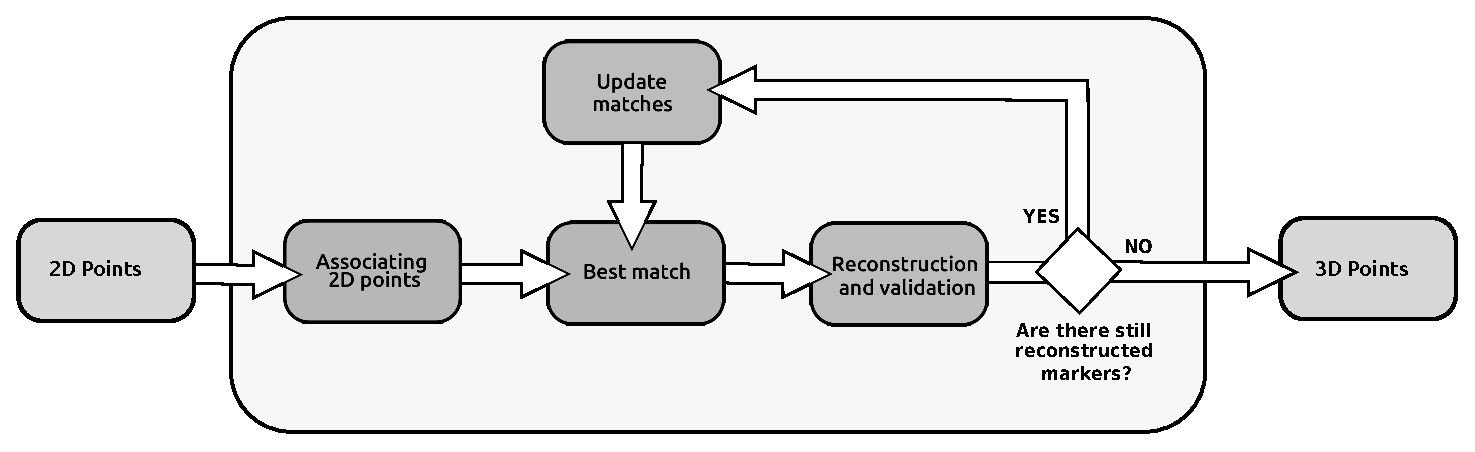
\includegraphics[scale=0.45]{./imagenes/Reconstruccion/bloques_reconstruccion}
        \caption{Block diagram of reconstruction algorithm.}
        \label{fig: diagrama algoritmo}
    \end{center}
\end{figure}
%\vspace{-0.6cm}

\textit{Associating 2D points.}\label{seccion_asociar2D_uno}
%
This block receives as input the coordinates of detected points and projection matrices of the cameras, returning to each point a list sorted by relevance of the existing partnerships with points on other cameras. \\ 
\textit{\hspace*{0.5cm}Best match.}\label{MejorAsociacion}
%
From the list of associations between pairs of cameras it is necessary to choose one that possesses more probability to form the pair corresponding to the projection of a 3D marker views on such images.
%
From each pair of cameras is taken the association which maintains the shorter distance and contains valid points, discarding the rest. 
\vspace{-0.65cm}
\begin{figure}
    \begin{center}
       \includegraphics[scale=1.0]{./imagenes/Reconstruccion/Algoritmo_reconstruccion}       
    \end{center}
\end{figure}
\vspace{-1.0cm}

To choice the pairs of cameras were considered two cases.
The first one evaluates each camera with all remaining and the second one considers the arrangement of cameras in space and match the adjacent cameras consecutively.

\textit{3D reconstruction and Validation.}\label{seccion_reconstruccion3D_validacion}
Couple of points $x_i x_j$ of cameras $i$ and $j$ respectively, reconstruct a valid point 3D $X_{ij}$ if there is at least one $x_k$ in camera $k\not= i, \,j$ such that $X_{ik} \in $ sphere$(X_{ij}, \delta)$, to certain threshold $\delta$.

\textit{Update matches}\label{actualizar_asociaciones}
The couple who reconstructs $X_{ij}$ as well as $x_k$ points who validate this reconstruction are removed. 
Iteration continue repeating the process with next pairs of best associated cameras.
Finally iterative process stops when the number of reconstructed markers equals number of markers that the person has, equal to maximum number of reconstructions indicated, or not valid 2D points such that a partnership between different points of view can be established.
\subsection{Seguimiento}

The tracking of marker trajectories is performed by a sliding window of three or four frames linking the reconstructed points under the assumption that displacement of a marker from one frame into the next is minimal. This methodology was used by Herda \textit{et al.} \cite{herda} based on the work of Malik \textit{et al.} \cite{griegos}.

\hspace*{0.5cm} \textit{Algorithm}. Being known the trajectory of a marker until frame [f]  it's wanted to find the next position on frame [f+1] which is predicted by the displacement from [f-1] to [f]. A search neighbourhood is defined centered on the predicted point in which is expected to find the best reconstructed marker that continues the trajectory.

If within the search neighbourhood there is more than one posible candidate, for each of them is defined a second prediction on frame [f+2] such that the acceleration from [f-1], [f] and the predicted point in [f+1] is the same as the acceleration of [f+1] and the predicted point in [f+2]. Then is selected the trajectory whith the least variation of acceleration. If there is not any marker within the search neighbourhood  its radius is expanded up to a limit. If a trajectory could not be linked in a frame, the movement is prolonged into the next frames to find reconstructed markers near the predicted ones so the markers between those frames can be extrapolated. In addition, thresholds are implemented to define limits on the acceleration to detect discontinuities on the tracking. Figure \ref{restricciones_tracking} shows the motion capture of a walk standing out the trajectories of the leg markers.

\begin{figure}[ht!]
 \begin{center}
%  \subfloat[Trayectorias de marcadores de pierna]
  {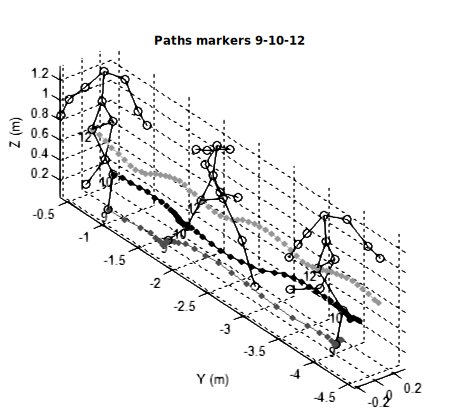
\includegraphics[scale=0.4]{imagenes/Seguimiento/050_Salida_Tracking_13_14_10} %\label{trayectorias_marcadores_piernas}
   }	
 % \subfloat[Distancia y Angulo entre marcadores de la pierna.]
 {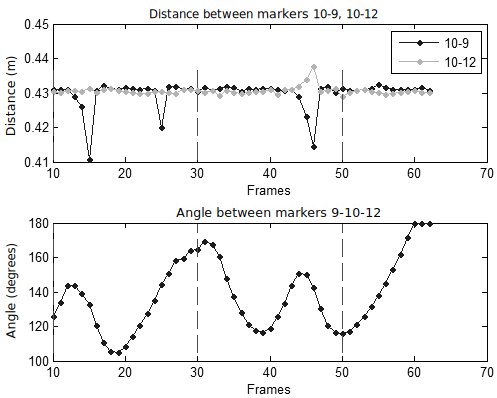
\includegraphics[scale=0.4]{imagenes/Seguimiento/051_Salida_Angulo_Distancia_13_14_10}\label{distancia_angulo_marcadores_piernas}}
  \end{center}
\caption{\textit{Left}: leg markers trajectories. \textit{Right}: distance and angle between two leg markers.}
\label{restricciones_tracking}
\end{figure}


Another tracking algorithms could be used like Kalman \cite{kalman} which requires the inicialization of models. There are also algorithms based on the constraint that some markers keep a constant distance between them.

%
%
%\subsection{Seguimiento}
%
%El seguimiento de trayectorias se realiza sobre una ventana deslizante de tres a cuatro cuadros enlazando los puntos reconstruidos de manera de mantener un movimiento lo mas suave posible. 
%Esta metodología fue utilizada por Herda \cite{herda} en su trabajo basándose en los estudios de Malik, Drako, Papantoniou \cite{griegos} .
%
%
%\hspace*{0.5cm} \textit{Algoritmo.} Sea la trayectoria de un marcador enlazada hasta el instante [f] sobre la cual desea buscarse su próximo punto en [f+1], el movimiento entre [f-1] y [f] es prolongado para establecer un centro de búsqueda y encontrar el punto reconstruido que mejor continúa la trayectoria como se muestra en la Figura \ref{herda_00} .
%
%%\vspace{-0.7cm}
%\begin{figure}[ht!]
%\begin{center}
%\includegraphics[scale=0.4]{imagenes/Seguimiento/tracking-eps-converted-to.pdf}
%\end{center}
%\caption{Seguimiento en cuatro cuadros, siendo [f] el cuadro actual que queremos seguir en [f+1]. ( Fuente  Human movement
%science 20(3), 313–341 \cite{herda} ) .}
%\label{herda_00}
%\end{figure}
%%\vspace{-0.3cm}
%Se presentan tres posibles casos al buscar puntos reconstruidos:
%
%\begin{itemize}
%
%\item Si solo se encuentra un punto reconstruido se agrega a la trayectoria para el cuadro [f+1], buscando el mas cercano a la estimación calculada como aquella que mejor se aproxima a una trayectoria de tres puntos con aceleración mínima
%
%\item En el caso de encontrar mas de un punto cada posible candidato es evaluado para realizar una segunda estimación hacia [f+2] de forma que la aceleración entre [f-1], [f] y el candidato en [f+1] sea la misma que entre [f], el candidato en [f+1] y la estimación en [f+2]. Luego de todos los posible caminos en cuatro cuadros, se elige el de menor variación de aceleración.
%
%\item Si no se encuentra ningún punto, se procede a aumentar de forma limitada el radio de búsqueda en [f+1] de forma excepcional. Esto se hace para continuar trayectorias que entran en estado de reposo y el último movimiento conocido es nulo o muy pequeño.
%
%\end{itemize}
%
%Si una trayectoria queda trunca durante el enlazado, se intenta recuperar prolongando el movimiento en próximas cuadros para encontrar puntos reconstruidos cercanos a las estimaciones y extrapolar los puntos intermedios. Por otro lado, se implementan umbrales para definir límites sobre la aceleración de los enlaces obtenidos y detectar discontinuidades durante el seguimiento.
%
%Estas medidas permiten detectar trayectorias individuales sobre los puntos reconstruidos, detectar de forma simple posibles discontinuidades, y estimar reemplazos en casos de pérdidas. La captura en la Figura \ref{restricciones_tracking} corresponde a la marcha y se resaltan las trayectorias individuales de puntos de la pierna así como un esqueleto simple generado para visualizar la evolución entre marcadores.\\
%%\vspace{-0.25cm}
%\begin{figure}[ht!]
% \begin{center}
%%  \subfloat[Trayectorias de marcadores de pierna]
%  {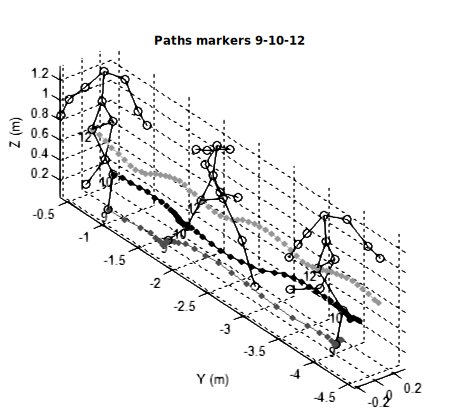
\includegraphics[scale=0.4]{imagenes/Seguimiento/050_Salida_Tracking_13_14_10} %\label{trayectorias_marcadores_piernas}
%   }	
% % \subfloat[Distancia y Angulo entre marcadores de la pierna.]
% {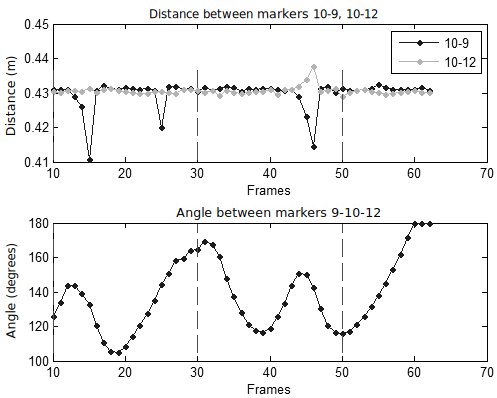
\includegraphics[scale=0.4]{imagenes/Seguimiento/051_Salida_Angulo_Distancia_13_14_10}\label{distancia_angulo_marcadores_piernas}}
%  \end{center}
%\caption{Posibles restricciones en ángulo y distancia, para el caso de la pierna en marcha. Izquierda: trayectorias de marcadores de pierna. Derecha: distancia y ángulo entre marcadores de la pierna.}
%\label{restricciones_tracking}
%\end{figure}
%%\vspace{-0.5cm}
%El conjunto de puntos reconstruidos puede ser sometido a otros algoritmos de seguimiento como Kalman \cite{kalman} requiriendo la inicialización de modelos, o algoritmos basados en restricciones más fuertes que utilicen las distancias relativamente constantes entre marcadores de los miembros y ángulos continuos entre articulaciones, requiriendo un mayor estudio de las características del sujeto y movimiento a capturar. %La Figura \ref{restricciones_tracking} muestra posibles restricciones en la marcha sobre los huesos de la pierna.
%
